\documentclass[11pt,a4paper,oneside]{report}
\usepackage[margin=1.0in]{geometry}
\usepackage{indentfirst}
\usepackage[pdftex]{graphicx}
\usepackage{wrapfig}


\pagestyle{empty}

\renewcommand{\thesection}{1}

\begin{document}
\begin{center}
\LARGE{ \bf IROS 2012 Travel Award Reimbursement Packet: Experience Report }
%\Large{Daniel M. Lofaro \\ }
%\large{Electrical and Computer Engineering Dept. \\ Drexel University \\ Philadelphia PA, USA \\}
%\large{\tt dml46@drexel.edu }
\end{center}

\section*{Student Information}
\begin{itemize}
\item Name: Daniel M. Lofaro - Electrical and Computer Engineering Dept. Drexel University
\item Student Status: Full-time Ph.D Student (see attached file)
\item Status: United States Citizen (see attached file)
\item Email: \tt{dml46@drexel.edu}
\end{itemize}


\section*{Paper Information}
\begin{itemize}
\item Number: 1255
\item Title: \textit{Humanoid Throwing: Design of Collision-Free Trajectories with Sparse Reachable Maps}
\item Description: Design, simulation and hardware testing of a method to create collision-free throwing trajectories for high degree of freedom manipulators. 
\end{itemize}


\section*{Keynote Summary: Gill Pratt}
Being a part of the DARPA Robot Challenge (DRC) I was especially interested in Gill Pratt's Keynote talk.  
At the time our team (DRC-Hubo) had been tentatively accepted to the Track-A part of the competition with official acceptance to come on October 26th.  
The talk gave us a chance to hear Gill announce further details and hints about the other competitors in Track-A.  
Though he did not state the names of any competitors directly Gill did hint at a foreign competitor that stepped down from their teaching positions to do this competition.  
This ended up being the SHAFT team from Tokyo University.  
In addition an important announcement was that the \textit{pump replacement} task might be changed with another task.
This ended up being tentatively replaced by \textit{hose/cable insertion}.  
Other than the latter, the rest of the presentation was about how DARPA is starting this competition as a direct response to the Fukushima disaster. 
He states that if one valve was turned the whole thing could have ended up different.
However we could not get humans close enough to turn it due to radiation levels.
He also mentioned that the robots we did send in could not traverse the stairs even through they were designed to do just that. 
This was because the robots were treaded (tank like) robots and the stairs had front edges that were rounded off due to years of human use.
Overall it was a nice informative talk

\section*{Summary of My Session}
I presented my work on \textit{Humanoid Throwing: Design of Collision-Free Trajectories with Sparse Reachable Maps}.  
This work shows how you can use a virtual model of a robot and pre-compute configurations that do not cause self collisions.  
The configurations consist of end effector locations in free-space and the corresponding joint-space configurations.  
The collection of N amount of configurations that do not contain a self collision form the Sparse Reachable Map or SRM.  
This map can be used in real-time to compute inverse kinematics on joints consisting of \underline{more than} 7-DOF.  
Inverse Jacobian IK is used to make a configuration for any free-space point close to but not directly in the SRM.
Though it can also be used for kinematic chains less than 7-DOF, they can be analytically solved for thus it is not needed.
Over all I was happy with the presentation especially because one of my colleagues from Samsung was there.
He works on their \textit{``new''} humanoid called RoboRoy (which was officially daubed at IROS 2012).
He said that there is a use for using an SRM for HRI or path planning in high-DOF robots.

\section*{Conference Experience Furthering Research and Career Agenda}

\begin{wrapfigure}{r}{0.5\columnwidth}
%\begin{figure}[thpb]
  \centering
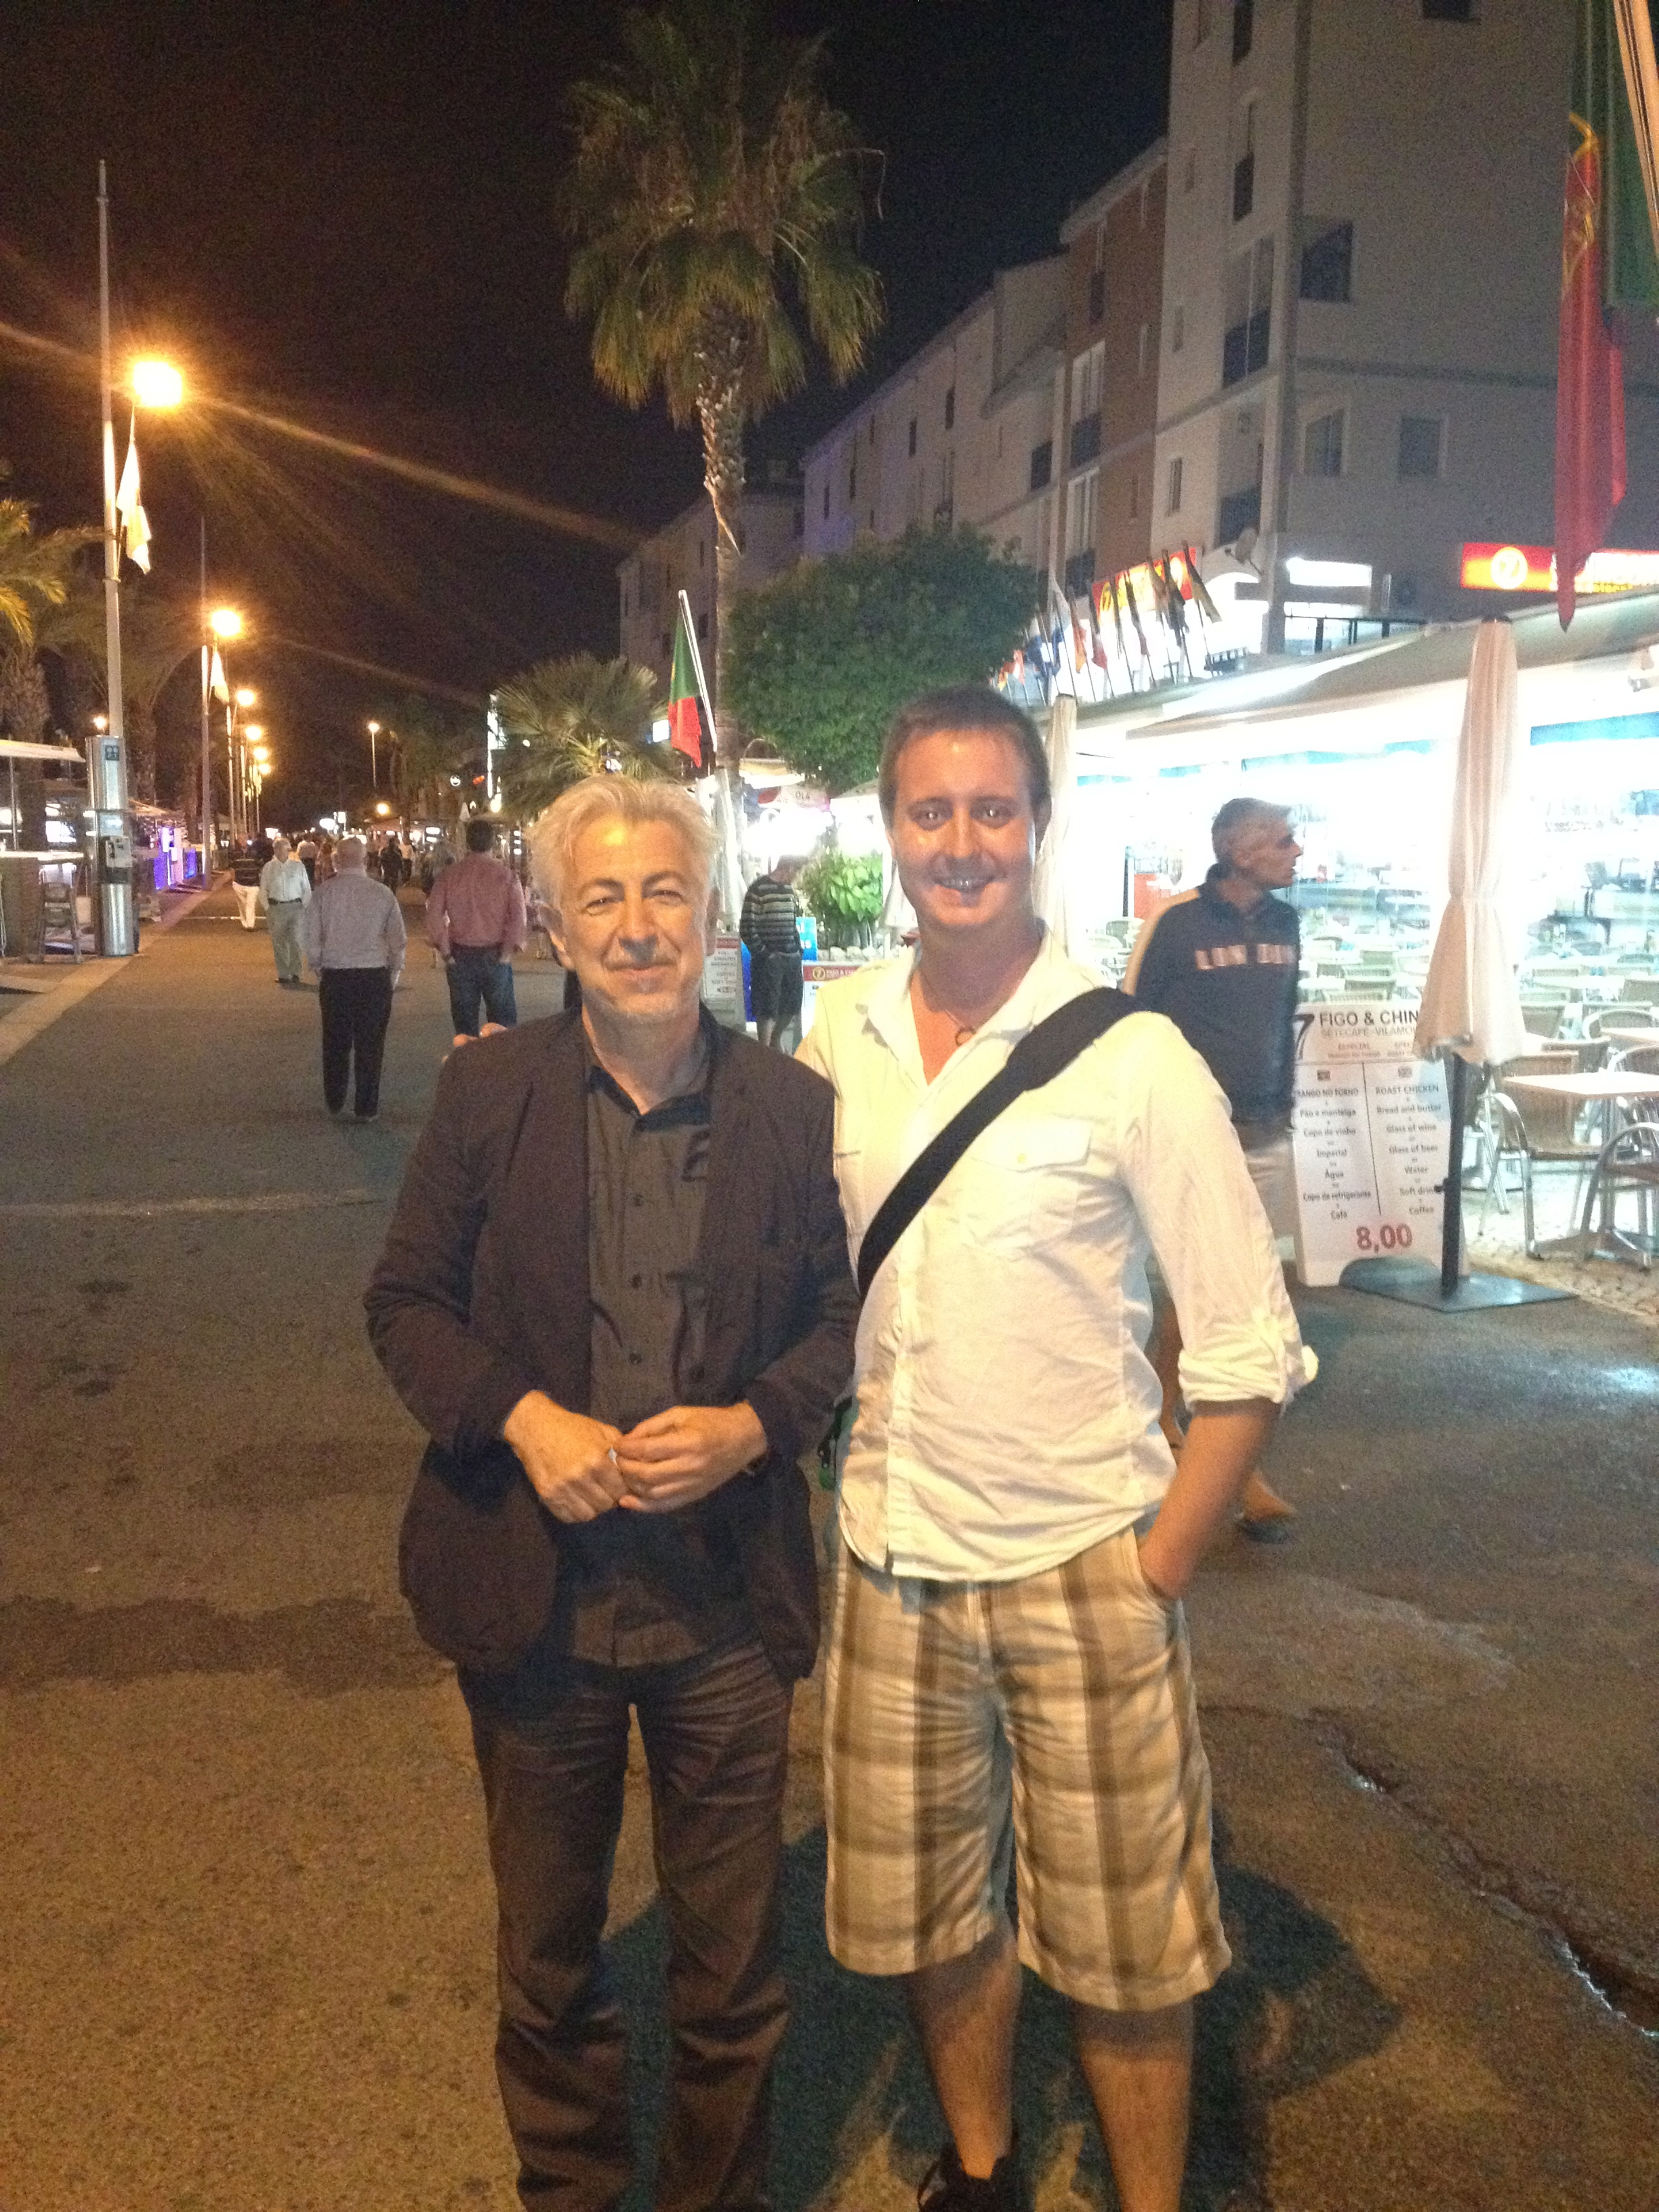
\includegraphics[width=0.5\columnwidth]{./IMG_1656.jpg}
  \caption{ Me and Dr. Oussama Khatib}
  \label{fig:graph}
%\end{figure}
\end{wrapfigure}

While attending IROS 2012 two very important things happened.  
First I met and became friends with Ms. Angelica Lim a writer for IEEE Spectrum.
This is important because she currently lives in Tokyo and as it happens I was slated to attend the IEEE-RAS Humanoids 2012 conference in Osaka, Japan in a few months (December 2012).
As I did for ICRA 2012 in May I was planning on making a variety of student events for Humanoids 2012.
My over all purpose for these events is to \textit{``create an atmosphere conducive for students to get to know each other in a non-academic setting.''}
After all these are the same people we will be working with for the next 40 years, we should all become friends.
Because ICRA was in the USA I knew people in the venue's location and had no problem setting up the events.
However because Humanoids was in Osaka, Japan I was having trouble with pre-planning for the events.
This is where meeting Angelica at IROS 2012 became a \underline{required part} of my planned student activities.
Angelica agreed to help me plan and organize the events.
She knew the area and the language which is key to making good events.
In fact if it was not for Angelica the events would \underline{not} have gone nearly as well.
The events consisted of:  \textit{daily group lunch and dinners for students}, \textit{Karaoke night}, a \textit{day trip to Kyoto}, and a \textit{Student Banquette}.
The students were very grateful that we put this event together.  
We got great reviews from both the students as well as from the faculty.
Pictures and descriptions of all of the events are available on the event's home page \textit{http://humanoids2012.danlofaro.com/}.
I can not stress enough that this event would \underline{\textbf{NOT}} have happened \underline{without the connections I made in IROS 2012}.

On more of a personal note; I have been a fan of Dr. Oussama Khatib's work at Stanford University for many years.
At IROS 2012 I had a chance to have dinner with Oussama on two occasions, both in a party of less then 6 people.  
This allowed us to talk about our common research on humanoids and put me on his \textit{``radar.''}
This is important because I am looking for faculty or post-doc positions as well as new collaborators.
We exchanged information and even went out for a drink.
I personally believe this will help me in the future because now I have a new connection for collaborative research.



\end{document}